\chapter{Programátorská dokumentace systému PerfEval}

\section{Architektura systému}

Architekturu systému PerfEval je možné rozdělit do~dvou částí. První část systému tvoří
parser příkazové řádky a~tzv. setup třídy. Druhou částí jsou tzv. command třídy,
které provádí skutečně požadovanou činnost. V~této části dokumentace nemusí být
některé podrobnosti o~implementaci, které je možné najít v~automaticky generované dokumentaci
JavaDoc. Jedná se například o~argumenty zmiňovaných metod.

Vnitřní struktura běhu je velice jednoduchá. Metoda \lstinline{main} má tři jednoduché úkoly.
Zavolat metodu \lstinline{getCommand} na~třídě \lstinline{Parser}. Tato metoda vrátí objekt typu \lstinline{Command},
na kterém metoda \lstinline{main} zavolá metodu \lstinline{execute}. Metoda \lstinline{execute} při návratu vrací enumerátor
typu \lstinline{ExitCode}. Na~objektu \lstinline{ExitCode} pak na~konci metoda \lstinline{main} zavolá metodu \lstinline[keywords={}]{exit},
která ukončuje program s~požadovaným exit kódem. Metody \lstinline{getCommand} a~\lstinline{execute} mohou skončit
s~výjimkami \lstinline{ParserException} a~\lstinline{PerfEvalCommandFailedException}. Pro tyto případy tyto
výjimky obsahují položku \lstinline{exitCode}, na~které metoda \lstinline{main} opět zavolá metodu \lstinline[keywords={}]{exit}.

\subsection{Použité návrhové vzory}

Součástí architektury systému PerfEval je několik běžných návrhových vzorů.
Prvním z použitých návrhových vzorů je factory. Factory je použitý
při práci s parsery vstupních souborů. Factory třídou podle tohoto návrhového vzoru je
zde třída \lstinline{ParserFactory}. Tato třída konstruuje parsery podle parametru metody
\lstinline{getParser}.

\begin{figure}[!ht]
    \centering
    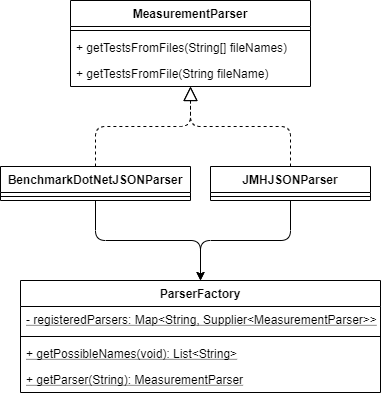
\includegraphics[width=0.5\textwidth]{../img/architektura-factory.png}
    \caption{Struktura části PerfEvalu - návrhový vzor factory}
\end{figure}


Druhým použitým návrhovým vzorem je builder. Jednotlivé builder třídy
jsou implementacemi rozhraní \lstinline{CommandSetup}. Tyto builder třídy v~rámci
systému PerfEval v~rámci metody setup konstruují objekt typu \lstinline{Command}.

\begin{figure}[!ht]
    \centering
    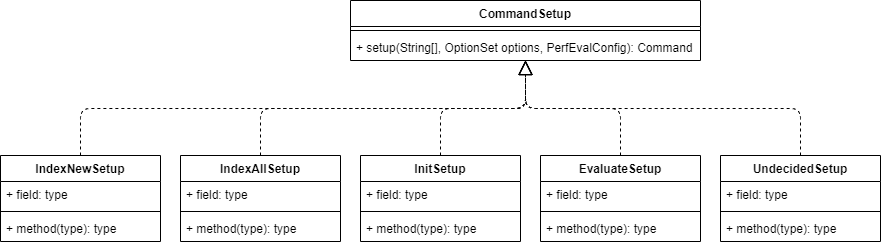
\includegraphics[width=0.9\textwidth]{../img/architektura-builder.png}
    \caption{Struktura části PerfEvalu - návrhový vzor builder}
\end{figure}

Dalším použitým návrhovým vzorem je strategy. Tento návrhový vzor je využitý při
volbě statistického testu, který se bude používat pro vyhodnocení, a pro volbu toho,
jakou podobu výstupu má program vyrobit. Na obrázku s~příkladem tříd jsou vidět
jednotlivé strategie pro volbu formy výstupu.

\begin{figure}[!ht]
    \centering
    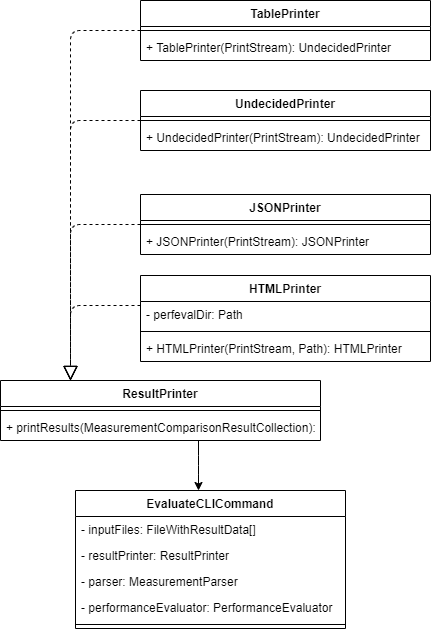
\includegraphics[width=0.6\textwidth]{../img/architektura-strategy.png}
    \caption{Struktura části PerfEvalu - návrhový vzor strategy}
\end{figure}

Posledním použitým návrhovým vzorem je návrhový vzor command. Protože je PerfEval
konzolová aplikace ovládaná pomocí příkazů, tak je příhodné jej použít. Na~obrázku
jsou vidět dostupné implementace rozhraní \lstinline{Command}. Pro každý z~příkazů
systému PerfEvalu se zkonstruuje nějaká jeho implementace a~na ní se zavolá její metoda
\lstinline{execute}.

\begin{figure}[!ht]
    \centering
    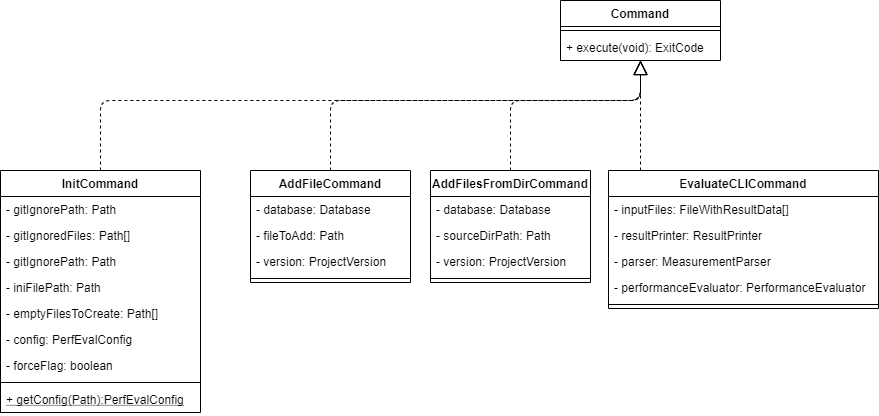
\includegraphics[width=0.9\textwidth]{../img/architektura-command.png}
    \caption{Struktura části PerfEvalu - návrhový vzor command}
\end{figure}

\subsection{Parser a setup třídy}

Třídu \lstinline{Parser} tvoří slovník \lstinline{commandPerSetup} a~metoda \lstinline{getCommand}.
Ve slovníku jsou k jednotlivým řetězcovým klíčům přiřazeny objekty typu
\lstinline{Supplier}, které mají za~úkol vracet instance typu \lstinline{CommandSetup}.
Klíče jsou skutečné řetězce zadávané uživatelem. \lstinline{Parser} pak na~základě příkazu
zadaného na~příkazové řádce zkonstruuje skrze \lstinline{Supplier} získaný ze~slovníku správnou
instanci třídy \lstinline{CommandSetup}. Na~této instanci se zavolá metoda \lstinline{setup}, která vrací
objekt typu \lstinline{Command}, podle definice rozhraní \lstinline{CommandSetup}. Metoda \lstinline{getCommand} je volaná
z~metody \lstinline{main}, která tvoří hlavní metodu programu.

Třída \lstinline{Parser} předává do~metody \lstinline{setup} objekty \lstinline{OptionSet}, které reprezentují argumetny příkazové řádky,
a~\lstinline{PerfEvalConfig}. Třída \lstinline{PerfEvalConfig}
reprezentuje globální konfiguraci systému PerfEval podle konfiguračního souboru.
\lstinline{Parser} tedy skrze statické metody této třídy zařídí přečtení konfiguračního souboru
do~objektu \lstinline{PerfEvalConfig}. Objekt \lstinline{OptionSet} reprezentuje parametry a~značky zadané
uživatelem na~příkazovou řádku. Jedná se o~objekt z~knihovny joptsimple. Rozpoznávány jsou
všechny značky blíže specifikované ve~třídě \lstinline{SetupUtilities}.

\lstinline{SetupUtilities} je třída obsahující statické položky a~řetězcové konstanty.
Tyto položky a~konstanty slouží pro~zpracování argumentů příkazové řádky.
Setup třídy a~\lstinline{Parser} využívají jednotlivé metody této třídy.
Protože některé setup třídy využívají stejných metod ze~třídy \lstinline{SetupUtilities}, tak jsou tyto metody umístěny
právě ve~třídě \lstinline{SetupUtilities}.

\lstinline{InitSetup} je třída, která má za~úkol připravit instanci \lstinline{InitCommand}. Protože se jedná
o~setup třídu, tak připravuje data pro~práci instance typu \lstinline{Command}, který konstruuje. Poté, co v~rámci
metody \lstinline{setup} připraví potřebná data zkonstruuje \lstinline{InitCommand} a~vrátí jej.
Tímto je \lstinline{InitCommand} připraven k~práci.

\lstinline{IndexNewSetup} je třída pro přípravu instance \lstinline{AddFileCommand}. Tato setup třída dodává
při konstrukci instance \lstinline{AddFileCommand} cestu k přidávanému souboru, implementaci rozhraní \lstinline{Database}
a~instanci objektu \lstinline{ProjectVersion}. Instance objektu \lstinline{ProjectVersion} popisuje verzi softwaru pro kterou
byl nově přidávaný výsledek změřen. Zkonstruovanou instanci třídy \lstinline{AddFileCommand} vrací metoda \lstinline{setup}.

\lstinline{IndexAllSetup} je třída pro přípravu instance \lstinline{AddFilesFromDirCommand}. Té je při konstrukci dodána
implementace rozhraní \lstinline{Database}, cesta ke složce, ze které se budou přidávat soubory,
a~instance objektu \lstinline{ProjectVersion}. Instance objektu \lstinline{ProjectVersion} popisuje verzi softwaru pro kterou
byly nově přidávané výsledky změřeny. Zkonstruovanou instanci třídy \lstinline{AddFilesFromDirCommand} vrací metoda \lstinline{setup}.

\lstinline{EvaluateSetup} je třída která připravuje \lstinline{EvaluateCLICommand}. Tato setup třída musí v~databázi najít
soubory s~výsledky měření, které bude konstruovaný \lstinline{EvaluateCLICommand} porovnávat. Dále vyrábí správné
implementace rozhraní \lstinline{StatisticTest} a \lstinline{ResultPrinter}, podle argumentů z~příkazové řádky.
\lstinline{EvaluateSetup} musí vyrobit také instanci objektu \lstinline{PerformanceEvaluator}. Tuto instanci vyrobí
z~nastavení v~objektu \lstinline{PerfEvalConfig} a~ze~zmíněné implementace \lstinline{StatisticTest}. \lstinline{EvaluateCLICommand} je zkonstruovaný
z~vyrobených instancí \lstinline{PerformanceEvaluator}u, \lstinline{ResultPrinter}u, \lstinline{MeasurementParser}u a~vstupních souborů s~výsledky.
\lstinline{MeasurementParser} je součástí objektu \lstinline{PerfEvalConfig}.

\lstinline{UndecidedSetup} konstruuje \lstinline{EvaluateCLICommand} způsobem z~předchozího odstavce.
Jediný rozdíl je, že se použije pevně stanovený \lstinline{ResultPrinter} typu \lstinline{UndecidedPrinter}.
Tato implementace \lstinline{CommandSetup} vznikla proto, aby se vypsání informace o~nerozhodných
testech vypisovala pomocí odlišného příkazu.

Třída \lstinline{ListResultsSetup} připravuje instanci \lstinline{ListResultsCommand}. Jediná činnost metody setup
spočívá ve~vyrobení instance rozhraní \lstinline{Database}. Tuto instanci předá konstruktoru
třídy \lstinline{ListResultsCommand}. Vyrobenou instanci třídy \lstinline{ListResultsCommand} vrací.

\subsection{Command třídy}

V~této podkapitole je popsaný význam a práce jednotlivých implementací tozhraní Command.
Implementace třídy Command musejí mít implementovanou jedinou metodu \lstinline{execute}.

Třída AddFileCommand má~za~úkol přidat nový výsledek měření do~databáze. Vnitřní položky
třídy jsou fileToAdd, \lstinline{database} a~version. Metoda \lstinline{execute} tedy volá metodu addFile na dodané implementaci
databáze. Předávané parametry jsou fileToAdd a~version.

Třída \lstinline{AddFilesFromDirCommand} má~za~úkol přidat všechny výsledky měření ve složce do~databáze. Vnitřní položky
třídy jsou sourceDirPath, \lstinline{database} a~version. Metoda \lstinline{execute} tedy volá metodu addFilesFromDir na~dodané implementaci
databáze. Předávané parametry jsou sourceDirPath a~version.

%% nutno upravit implementaci -> detail
Třída \lstinline{InitCommand} má za~úkol v~adresáři, odkud byl PerfEval z~příkazové řádky spuštěn, inicializovat systém PerfEval.
Inicializace systému PerfEval probíhá v několika krocích. Nejprve se vytvoří adresář .performance. Následně se do~.gitignore
(v případě neexistence bude vytvořen) souboru doplní ignorace souborů a adresářů systému PerfEval. Nakonec je~z~parametrů
dodaných při~konstrukci a~z~výchozích parametrů vytvořen konfigurační soubor config.ini. V případě, že systém je
v~adresáři již inicializovaný a nebyl dodán příznak násilné inicializace, tak systém nebude inicializovaný.

Třída \lstinline{EvaluateCLICommand} má za~úkol porovnat výsledky měření výkonu dvou různých verzí.
Soubory s~výsledky dvou verzí a~parser k~nim jsou dodané při~konstrukci. Při~konstrukci
je dodaná implementace rozhraní \lstinline{StatisticTest}. Zmíněná instance slouží ke~statistickému
porovnání výsledků měření. Při~konstrukci je dále dodaná implementace rozhraní \lstinline{ResultPrinter}.
Implementace tohoto rozhraní rozhoduje o tom, jakým způsobem budou prezentovány výsledky porovnání.
Třída v rámci volání metody \lstinline{execute} nechá naparsovat soubory s výsledky měření do objektů typu \lstinline{Samples}.
Seznamy těchto objektů nechá porovnat pomocí statistického testu. Výsledkem je objekt MeasurementComparisonResultCollection.
Tento objekt je nakonec pomocí dodané implementace rozhraní \lstinline{ResultPrinter} prezentováno uživateli.

Třída \lstinline{ListResultsCommand} a~její metoda \lstinline{execute} slouží k~prostému vypsání obsahu databáze s~výsledky měření.
Databáze obsahuje informace o~výsledcích měření jako je cesta k~souboru a~popis verze. Tyto údaje vypíše
metoda print na~třídě FileInfoPrinter do~přehledné tabulky na~standardní výstup.

\subsection{Implementace rozhraní MeasurementParser}

Rozhraní \lstinline{MeasurementParser} je určeno ke~zpracování souborů s~výsledky měření výkonu.
Metoda \lstinline{getParser} třídy \lstinline{MeasurementFactory} vrací správnou instanci \lstinline{MeasurementParser}u na~základě dodaného jména (řetězce).
Jméno parseru je uloženo v konfiguračním souboru.

Implementace rozhraní mohou při zpracovávání souborů vyhazovat runtime výjimku
\lstinline{MeasurementParserException}. Výjimka je odchytávaná mimo implementaci \lstinline{MeasurementParser}
v~metodě \lstinline{execute} třídy \lstinline{EvaluateCLICommand}. Výjimku je tedy bezpečné vyhazovat.

Aktuálně dostupné implementace rozhraní \lstinline{MeasurementParser} jsou pouze dvě.
\lstinline{JMHJSONParser}, který umí zprácovavat výstup frameworku JMH ve~formátu JSON, a \lstinline{BenchmarkDotNetJSONParser}, který
umí zprácovavat výstup frameworku BenchmarkDotNet ve~formátu JSON.

\subsection{Implementace rozhraní StatisticTest}

Rozhraní \lstinline{StatisticTest} definuje, jaké metody mají mít implementace statistických testů
pro porovnání dvourozmětných polí typu double. Jedná se o~metodu, která vrací interval spolehlivosti.
Interval spolehlivosti je intervalový odhad střední hodnoty pro rozdíl dvou náhodných veličin.
Dále musí umět vrátit odhad minimálního počtu vzorků, které jsou zapotřebí pro zajištění dostatečně úzkého intervalu.

Implementace tohoto rozhraní jsou dvě. První je třída \lstinline{ParametricTest}, která používá
Welchův t-test, který je podrobněji popsán v~kapitole 2.3.1. Druhou implementací je
\lstinline{NonparametricTest}, který využívá hierarchického bootstrapu. Tento bootstrap je podrobněji
popsaný v~kapitole 2.3.2.

\subsection{Implementace rozhraní Database}

Rozhraní \lstinline{Database} definuje funkce, které jsou požadovány od~systému, který má ukládat
metadata o~výsledcích měření. Jeho jediná implementace využívá technologie H2 embedded databáze.
Technologie umožňuje vyhledávat položky v~lokální databázi pomocí standardních SQL příkazů.

\section{Rozšiřitelnost a její omezení}

Systém PerfEval byl od~počátku projektován tak, aby byl rozšiřitelný.
V~různých částech návrhu se~vyskytují místa,
kde je možné významným způsobem doplnit a~změnit chování celé aplikace.

Nejdůležitější ze~zmiňovaných rozšíření je rozšíření o~datový formát. Tato možnost dělá z~PerfEvalu
poměrně univerzální nástroj. Činí ho totiž méně závislým na~použitém měřícím systému a~jeho výstupním formátu.

\subsection{Rozšíření o datový formát}

Vezměme opět scénář našeho programátora z~první kapitoly. Programátor si napsal výkonnostní testy.
Testy napsal pomocí nástroje, který nepodporuje PerfEval. Nicméně progrmátor ví, že~systém PerfEval
dělá přesně to, co~potřebuje. Jediný problém je tedy ve~vysvětlení svého datového formátu systému.

PerfEval je od~počátku zamýšlen pro rozšíření v~tomto místě. Programátor tedy musí prozkoumat, jak správně zkonstruovat
třídu \lstinline{Samples}. Třída \lstinline{Samples} obsahuje všechny hodnoty naměřené pro jednu testovanou metodu a~instanci
třídy \lstinline{Metric}. Instance třídy \lstinline{Metric} reprezentuje fyzikální jednotku a~příznak jestli vyšší hodnota
znamená vyšší výkon.

Programátor musí naimplementovat rozhraní \lstinline{MeasurementParser}. V~tomto rozhraní je důležitá metoda
\lstinline{getTestsFromFiles}. Tato metoda na~vstupu přijme všechny soubory s~výsledky měření jedné verze. Výstupem je list objektů
typů \lstinline{Samples}. Pro každou metodu (test výkonu), který se v~souborech nachází, se v~listu vyskytuje pouze jedna instance
typu \lstinline{Samples}.

Poslední krok tohoto rozšíření po~naimplementování \lstinline{MeasurementParser}u je jeho registrace. Registrace probíhá tak,
že~se~přidá jeden řádek do~statického konstruktoru třídy \lstinline{ParserFactory}. Na~řádku bude přidání položky do~objektu
s~názvem \lstinline{registeredParsers}. Tento objekt je typu \lstinline{HashMap} a~přiřazuje k~sobě \lstinline{Supplier}, který vrací \lstinline{MeasurementParser},
a~název typu \lstinline{String}. Přidávaná položka je tedy \lstinline{String} odpovídající názvu parseru a~reference na~metodu,
která umí parser zkonstruovat.

Použití nového parseru je pak jednoduché. Při inicializaci systému PerfEval příkazem init se jako argumentu
benchmark-parser použije jméno nového parseru. Dokonce jej začne hlásit v~nabídce i~chybová hláška v~případě, že žádný parser
není při~inicializaci zadán.

\subsection{Rozšíření o komparátor}

Pokud uživatel chce  PerfEvalu změnit pořadí výpisu testů~na výstupu, může použít komparátor.
Pokud mu žádný z~připravených nevyhovuje, tak může implementovat nový komparátor.
Tento komparátor je objektem typu Comparator, který porovnává instance MeasurementComparisonRecord. Pomocí tohoto
komparátoru, pak dojde k~setřídění vypisovaných prvků.

Dále je nutné přepsat metodu resolvePrinterForEvaluateCommand takovým způsobem, aby~reagovala i~na~nový druh komparátoru
podle příkazové řádky. Tuto metodu je možné nalézt ve~třídě \lstinline{SetupUtilities}.
Posledním krokem je přidání nové značky do~parseru příkazové řádky v~metodě createParser.
Komparátor se~pak může předávat objektům typu \lstinline{ResultPrinter} při~konstrukci.
O~jejich dalším použití si tedy tyto objekty rozhodují samy.

\subsection{Rozšíření o statistický test}

Může se stát, že~uživatel systému PerfEval má o~svých datech nějaké předpoklady, které
by chtěl při~vyhodnocování zohlednit. Může si tedy naprogramovat vlastní implementaci
rozhraní \lstinline{StatisticTest}, kde tyto předpoklady zohlední.

Po~naprogramování vlastní implementace rozhraní \lstinline{StatisticTest}, pak jen stačí ve~třídě \lstinline{SetupUtilities}
změnit chování metody resolve\lstinline{StatisticTest} tak,~aby~rozpoznnávala novou implementaci podle příkazové řádky. Posledním krokem je
přidání nové značky do~parseru příkazové řádky v~metodě createParser.

\subsection{Rozšíření o možnost výpisu}

Pro vypisování výsledků porovnání slouží rozhraní \lstinline{ResultPrinter}. Pokud by si uživatel chtěl naimplementovat
vlastní způsob vypisování, tak stačí implementovat jedinou jeho metodu PrintResults.

Přidání nového \lstinline{ResultPrinter}u je podobné jako rozšíření o~statistický test.
Je nutné změnit metodu \lstinline{resolvePrinterForEvaluateCommand} tak, aby vracela
i~novou implementaci \lstinline{ResultPrinter}u. Zmíněná metoda se nachází ve třídě
\lstinline{SetupUtilities}.
Pokud by~bylo zapotřebí nového argumentu na~příkazové řádce, tak je nutné do~metody \lstinline{createParser} jeho použití také
správně implementovat.

\subsection{Rozšíření o novou HTML šablonu}
Při použití přepínače \lstinline{html-output} bude výsledek porovnání uložen v~podobě HTML souboru.
Tento soubor je možné otevřít v běžném internetovém prohlížeči. Přepínač je možné doplnit o~argument
\lstinline{html-template}, kde bude uvedena cesta k nové šabloně. Dodaná šablona bude
ve formátu, který podporuje šablonový procesor Thymeleaf. Šabloně bude dodaná instance objektu
\lstinline{MeasurementComparisonResultCollection} jehož struktura je zdokumentovená v~JavaDoc
dokumentaci systému PerfEval.

\subsection{Změna použitého databázového systému}

V~důsledku rozhodování se o~tom, jak se budou informace o~výsledcích měření ukládat, vzniklo rozhraní \lstinline{Database}.
Rozhraní má mnoho metod. Pokud by se uživatel rozhodl změnit způsob ukládání dat o~měřeních, tak by
musel implementovat celé toto rozhraní. Po~implementaci rozhraní pak už jen stačí změnit metodu \lstinline{constructDatabase} ve~třídě
\lstinline{SetupUtilities}, která vrací instanci objektu typu \lstinline{Database}.

\subsection{Rozšíření o příkaz}

Každý příkaz PerfEval se skládá ze~dvou tříd. Jedná se o~třídu implementující rozhraní \lstinline{CommandSetup}
a~o~třídu implementující rozhraní \lstinline{Command}. Pokud by uživatel chtěl doplnit nějaký nový příkaz,
který by v~kontextu systému dával smysl, tak je to možné. Dobrý příklad pro~reprezentování nového příkazu
bude vyhodnocení výkonu s~grafickým výstupem.

Na~rozdíl od~stávajícího vyhodnocování by~grafické vyhodnocování potřebovalo údaje z~více než dvou posledních verzí.
Proto by příkaz evaluate-graphical metoda \lstinline{getCommand} rozpoznala jako příkaz a~vytvořila instanci nové setup třídy \lstinline{EvaluateGraphicalSetup}.
Na~této třídě, implementaci \lstinline{CommandSetup}, by pak zavolala metodu \lstinline{setup}. Metoda setup na~třídě \lstinline{EvaluateGraphicalSetup}
by měla za~úkol z~konfigurace PerfEvalu a~příkazové řádky vyrobit instanci nové třídy \lstinline{EvaluateGraphicalCommand}. Tuto instanci, která
by implementovala rozhraní \lstinline{Command}, by pak metoda \lstinline{getCommand} na~třídě \lstinline{Parser} vrátila.

Zbytek programu by se již nezměnil a~metoda \lstinline{main} ve~třídě \lstinline{Main} by vykonala dodaný příkaz. Spustila by~standardním způsobem
metodu \lstinline{execute} na~instanci objektu typu Command.

Zaregistrování nového příkazu by probíhalo přidáním nové položky do~statického konstruktoru třídy \lstinline{Parser}.
Položka mapy \lstinline{commandPerSetup} má obdobnou strukturu jako v~případě rozšíření o~nový \lstinline{MeasurementParser}.
Dodal by se řádek s~názvem příkazu typu \lstinline{String} a~z~reference na~bezparametrický konstruktor
implementace rozhraní \lstinline{CommandSetup}. Název příkazu odpovídá příkazu, kterým se bude volat z~příkazové řádky.

\subsection{Omezená rozšiřitelnost ve vyhodnocování}

Jeden z nejhorších požadavků na rozšíření systému by bylo rozšíření v oblasti vyhodnocování.
Jedná se o~změnu implementace třídy \lstinline{PerformanceEvaluator}. Tato třída utváří
celkovou vyhodnocovací logiku. Její rozšiřitelnost je omezená na implementace rozhraní
\lstinline{StatisticTest}.

Omezenou změnu chování vyhodnocování výkonnostních testů provést lze. Omezené změny ve~vyhodnocování
se provádí změnami hodnot uvnitř config.ini souboru.